\documentclass{../../slides-style}

\slidetitle{Практика, архиватор Хаффмана}{03.11.2023}

\begin{document}

    \begin{frame}[plain]
        \titlepage
    \end{frame}

    \section{Замечания по домашкам}

    \begin{frame}
        \frametitle{Замечания по домашним работам (1)}
        \begin{itemize}
            \item Внутренние функции модуля --- static
            \begin{itemize}
                \item Это делает функции невидимыми для линковщика вне модуля
                \item Бывают ещё static-переменные --- не очищаются при выходе из функции
                \item См. \url{https://en.cppreference.com/w/c/language/storage_duration} для тайных знаний
            \end{itemize}
            \item Явно приводите указатель к нужному типу после malloc/calloc и т.п.
            \item Не выделяйте большие массивы на стеке!
            \item Сдавайте задачи только пуллреквестами
            \item Всё, что по смыслу размер или индекс --- size\_t
            \item Подключайте нужные хедеры
            \begin{itemize}
                \item Например, string.h для strcmp
            \end{itemize}
        \end{itemize}
    \end{frame}

    \begin{frame}
        \frametitle{Замечания по домашним работам (2)}
        \begin{itemize}
            \item Константные указатели: \mintinline{c}{const Type * const}
            \item \mintinline{c}{var++} vs \mintinline{c}{++var}
            \item Используйте модули везде
            \begin{itemize}
                \item Тесты в отдельном модуле
                \item Структуры данных в отдельном модуле
                \item Файловый ввод-вывод (и сложный UI) в отдельном модуле
                \item Бизнес-логика (код, который собственно решает задачу) --- в отдельном модуле
                \item И main
            \end{itemize}
            \item Читабельные имена веток/PR на английском, никакого транслита
            \item Не коммитьте лишние файлы!
            \item Не дублируйте код
            \item И главное --- не сдавайте новые задачи, не поправив старые и повторяя старые ошибки
        \end{itemize}
    \end{frame}

    \begin{frame}[fragile]
        \frametitle{Замечания по домашним работам (3)}
        \begin{itemize}
            \item Замер времени:
            \begin{minted}{c}
typedef int *(SortMethod)(size_t const * const, size_t);

double calcDuration(SortMethod method, const * const array, 
    const size_t arraySize) 
{
    ...
}
            \end{minted}
            \item Примеры: \url{https://learnc.info/c/function_pointers.html}
            \item Чтение строк произвольной длины:
            \begin{itemize}
                \item \url{https://programforyou.ru/poleznoe/effektivnoe-poluchenie-stroki-proizvolnoj-dliny-na-c-i-c-plus-plus}
            \end{itemize}
            \item Можно сделать \mintinline{c}|string {char *data, size_t size, size_t capacity}| и читать в неё (автоматически реаллоцируя по необходимости)
        \end{itemize}
    \end{frame}

    \section{Задача}

    \begin{frame}
        \frametitle{Напоминание идеи алгоритма}
        \begin{columns}
            \begin{column}{0.5\textwidth}
                \begin{itemize}
                    \item Считаем частоты символов во входной строке
                    \item Склеиваем два самых редких в один псевдосимвол, пока не получили одно дерево
                    \item Строим по дереву префиксный код в виде таблицы
                    \item Бежим по строке, заменяя символ на его код
                    \begin{itemize}
                        \item Используем битовый буфер для формирования байта выдачи
                    \end{itemize}
                    \item При разархивировании бежим от корня до листа
                \end{itemize}
            \end{column}
            \begin{column}{0.5\textwidth}
                \begin{figure}[htp]
                    \centering
                    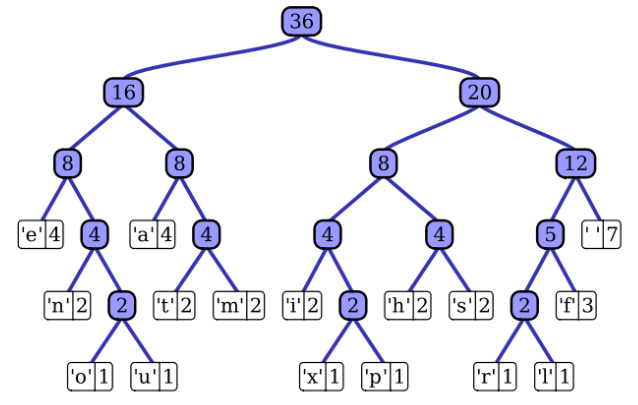
\includegraphics[width=0.8\textwidth]{huffman-tree.png}
                    Пример: ``this is an example of a huffman tree''
                \end{figure}
            \end{column}
        \end{columns}
    \end{frame}

    \begin{frame}
        \frametitle{Задача}
        \begin{enumerate}
            \item Описать двоичное дерево, хранящее символы и частоты, в отдельном модуле
            \item Построить дерево частот
            \item Построить таблицу с префиксными кодами
            \item (*) Получить сжатую строку
            \item (*) Оценить степень сжатия
            \item (*) Реализовать разжатие
        \end{enumerate}
    \end{frame}

\end{document}